\documentclass[11pt]{article}
 
\usepackage[a4paper, 
 	width = 120mm,
 	height = 220mm]{geometry}

\usepackage{color}
\definecolor{SU}{RGB}{0, 46, 95}
\usepackage{graphicx}

\usepackage{booktabs}

\usepackage{microtype}
 	
\usepackage{hyperref}
\hypersetup{
 	colorlinks,
 	citecolor = black,
 	filecolor = black,
 	linkcolor = SU,
 	urlcolor = SU,
 	pdfauthor = {Leonard Blaschek},
 	pdftitle = {Bio-informatics guide},
 	pdfkeywords = {Lignin methods}
}
 
\title{A quick guide to colony counting in \textsc{Fiji}}
 
\author{Leonard Blaschek}
 
\begin{document}
 	\maketitle
 	
 	\section*{Considerations before you start}
	This quick step-by-step guide will allow you to count colonies from pictures of agar plates.  As with most automated methodology, the precision and accuracy depends primarily on the quality of the input. Make sure that the colonies are large enough to be clearly visible, sparse enough to prevent adjacent colonies from overlapping, and that the picture has an even illumination and background.
 	
 	\section*{The counting procedure}
 	Once you have appropriate pictures, the procedure is as follows:
 	\begin{enumerate}
 		\item If not already done, download the \textsc{ImageJ} distribution \href{https://imagej.net/Fiji/Downloads}{\textsc{Fiji}}
 		\item Start \textsc{Fiji} and open the plate image
 		\item Make a circular selection of the whole plate; press \texttt{T} to save the selection in the ROI manager, and press \texttt{M} to measure it's area
 		\item Make a circular selection of a part of the plate that is free of writing and edges (aim for roughly 40--75\% of the whole plate); again, press \texttt{T} and then \texttt{M}; make sure to maintain this selection for the next two steps
 		\item Do \texttt{Edit $\rightarrow$ Clear Outside} to remove everything from the picture except the selected region of the plate
 		\item Do \texttt{Process $\rightarrow$ Binary $\rightarrow$ Make Binary} to transform the picture into black (colonies) and white (background); if the colonies are white on a black background, do \texttt{Edit $\rightarrow$ Invert}
 		\item Do \texttt{Process $\rightarrow$ Binary $\rightarrow$ Watershed} to separate overlapping colonies into individual spots
 		%\item Make a new circular selection the size of a single colony; press \texttt{M} to measure and note down the area
 		\item Go to \texttt{Analyze $\rightarrow$ Analyze Particles...}
 		%\item In the newly opened window, set the expected size of the colonies (\texttt{Size (pixel\textasciicircum2)}) according to the size of the colony you measured in step 8; set the range generously, \textit{e.g.} if you measured an area of 300 px, set the range to 100--1500 px
 		\item Leave \texttt{Circularity} at 0--1, select \texttt{Overlay Masks} from the \texttt{Show:} dropdown menu, and tick the \texttt{Summarize} and \texttt{In situ Show} boxes
 		\item Click \texttt{OK}
 		\item In the new \texttt{Summary} window, you see the number of counted colonies under \texttt{Count}; the counted colonies will appear coloured in the image, pixels that were ignored in the counting remain black (see figure 1)
 		\item Finally, extrapolate the number of total colonies on the plate using the areas measured in steps \textbf{3} and \textbf{4}.
 	\end{enumerate}
 
 \begin{figure}
 	\centering
 	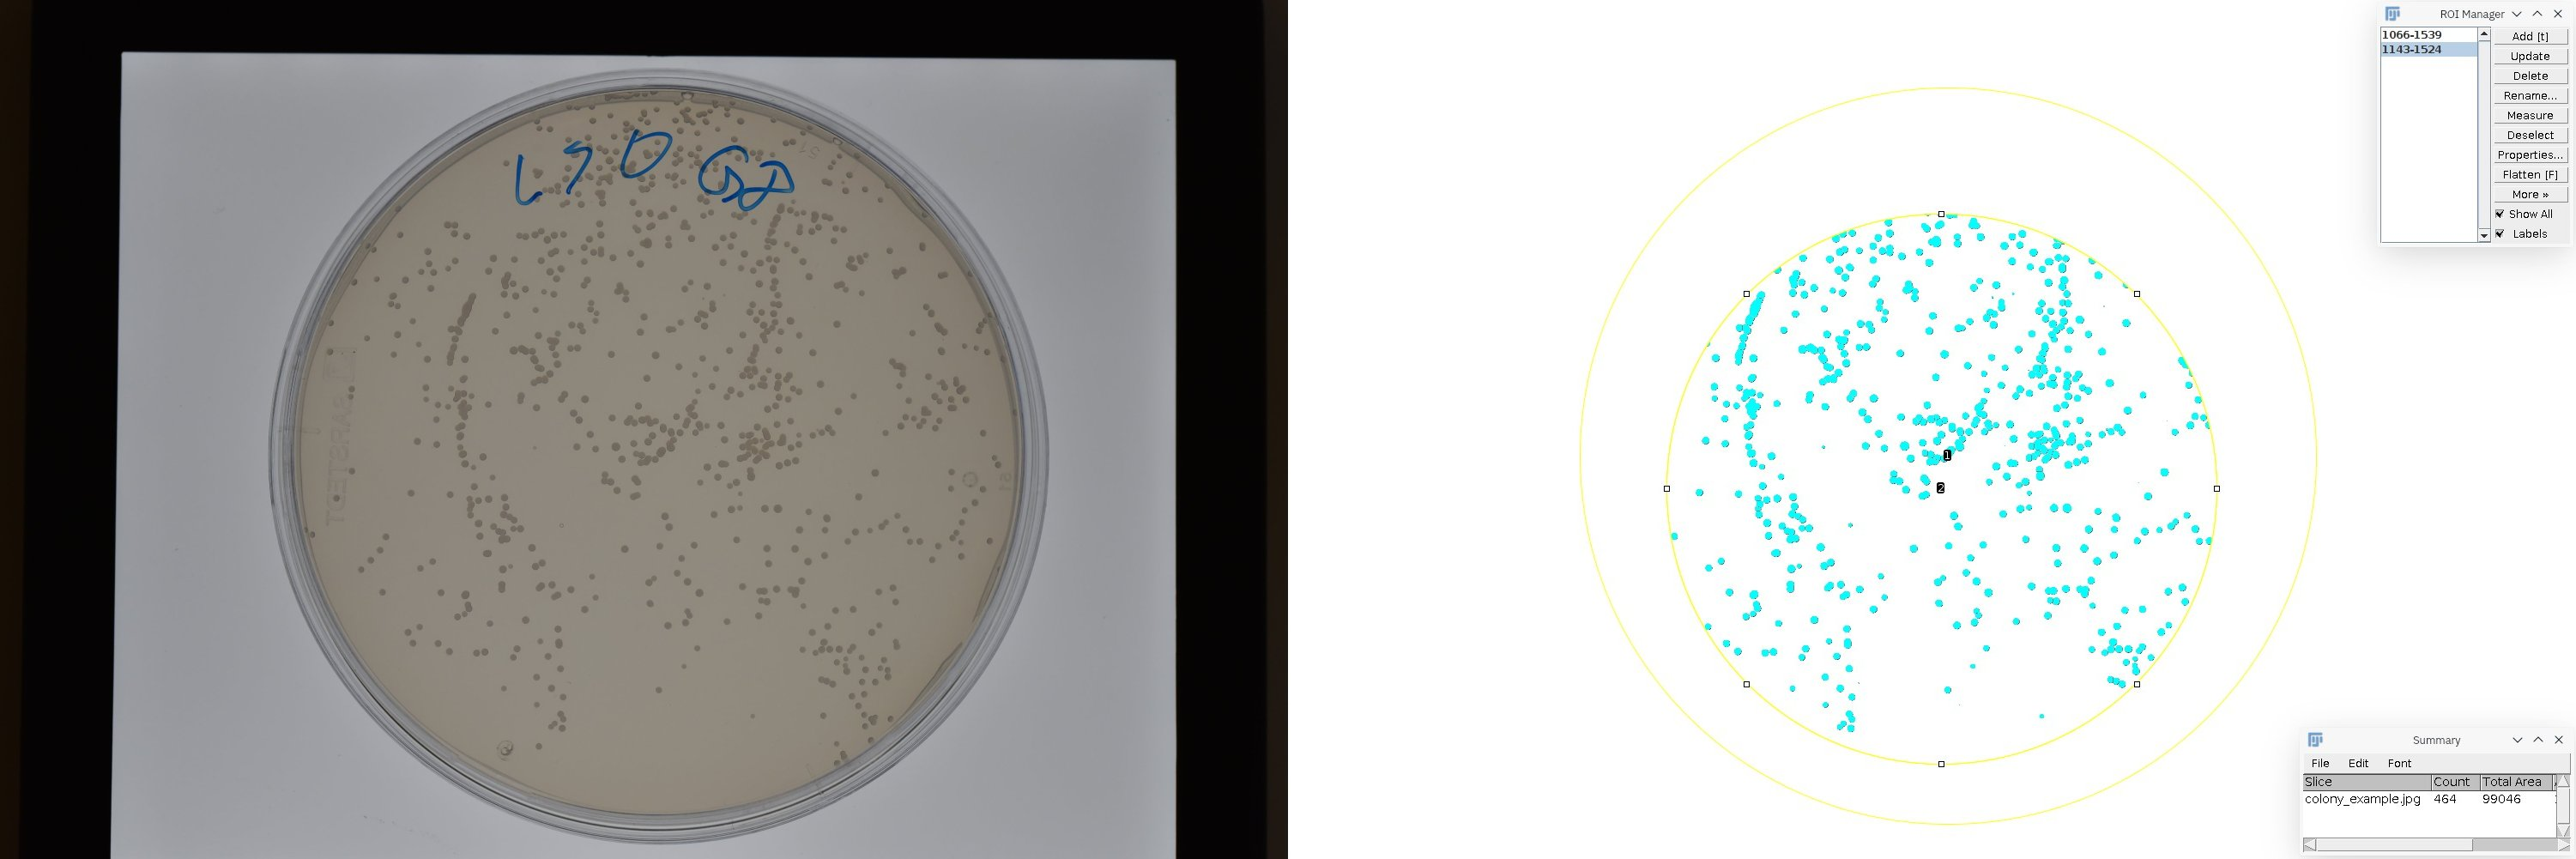
\includegraphics[width=0.95\linewidth]{colony_montage}
 	\caption[Example output.]{Example image of a bacterial plate (left), and the same plate after processing (right). In the right image, the large yellow circle is the selection created in step \textbf{3}, and the smaller yellow circle the selection created in \textbf{4}}
 	\label{fig:colonymontage}
 \end{figure}

\noindent\textit{Note: This tutorial covers only simple counting and area measurements. If you want to characterise additional parameters of the colonies such as colony shape, colour or heterogeneity, we just need to tweak a handful of steps. Let me know, and we can go through that together.}
 
 		
\end{document}
